\chapter{Schiemannen}
\vspace{-120px}
\question{1}{Met welke knoop maak je twee touwen van gelijke dikte aan elkaar vast?}
\answerTextFour{Schootsteek}{Paalsteek}{Constrictor}{Platte knoop}

\question{2}{Welke knopen zie je in de afbeelding hiernaast?}
	\vspace{-20px}
\begin{figure}[H]	

	\begin{minipage}[]{0.59\textwidth}
		\begin{enumerate}[topsep=0pt, label=\Alph*.]
			\item Links: platte knoop, rechts: een halve steek
			\item Links: achtknoop, rechts: schootsteek
			\item Links: reefsteek, rechts: dubbele halve steek
			\item Links: platte knoop, rechts: dubbele schootsteek
		\end{enumerate}
	\end{minipage}
	\begin{minipage}[]{0.20\textwidth}
	\begin{figure}[H]
		
\includegraphics[width=\textwidth,right]{Hoofdstukken/Schiemannen/pdf/platteknoop.pdf}
	\end{figure}
\end{minipage}
	\begin{minipage}[]{0.20\textwidth}
		\begin{figure}[H]
			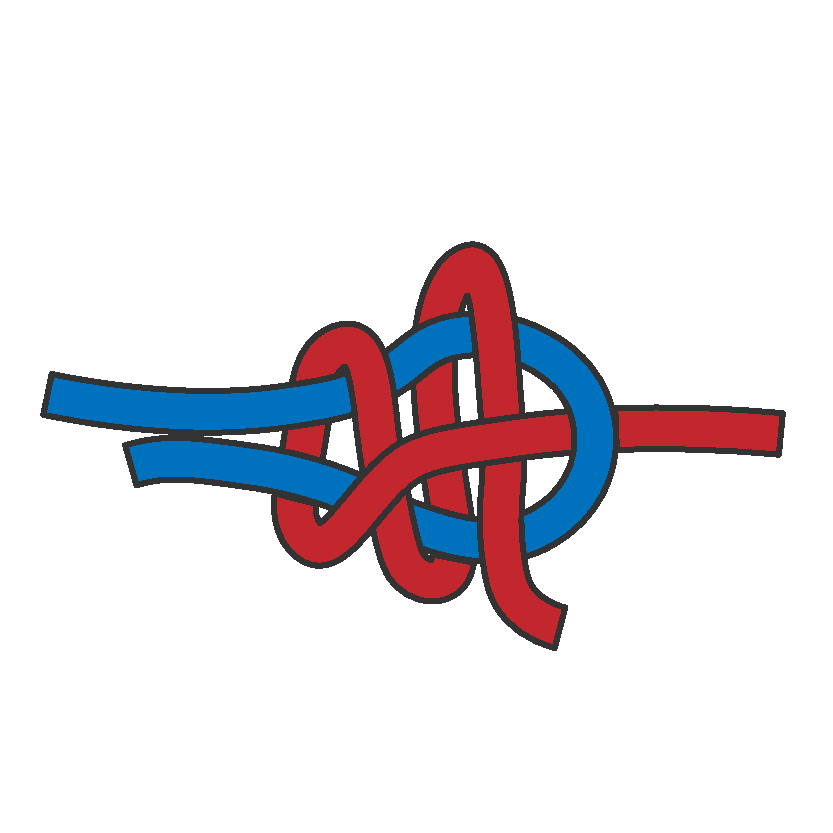
\includegraphics[width=\textwidth,right]{Hoofdstukken/Schiemannen/pdf/dubbele_schootsteek.pdf}
		\end{figure}
	\end{minipage}
	\vspace{-20px}
\end{figure}

\question{3}{Welke knoop laat een dubbele halve steek zien?}

\answerPicture{Hoofdstukken/Schiemannen/pdf/dubble_halve_steek_slippend.pdf}{Hoofdstukken/Schiemannen/pdf/paalsteek.pdf}{Hoofdstukken/Schiemannen/pdf/dubble_halve_steek.pdf}{Hoofdstukken/Schiemannen/pdf/halve_steek.pdf}



\question{4}{Met welke knoop leg je een niet-slippende lus in een lijn?}
\answerTextFour{Schootsteek}{Paalsteek}{Dubbele slipsteek}{Dubbele halve steek}

\question{5}{Welke stelling is waar?}
\answerTextFour{Natuurvezel kan beter tegen UV en heeft een hogere breeksterkte dan kunstvezel}{Kunstvezel heeft minder rek en is gevoeliger voor schavielen dan natuurvezel}{Natuurvezel is slijtvaster en heeft minder rek dan kunstvezel}{Kunstvezel kan beter tegen UV en is slijtvaster dan natuurvezel}

\question{6}{Bij welke lijn is enige mate van rek gunstig?}
\answerTextFour{Landvasten en ankerlijn}{Vallen}{Schoten}{Rijglijn}

